% CONSTRUCTING \& INTERPRETING LINEAR MODELS - WORKSHEET 0 (IN-CLASS INSTRUCTION)
\documentclass[12pt, letterpaper, fleqn]{article}

% ----------------------------------------------------------
% PACKAGES
% ----------------------------------------------------------
\usepackage{graphicx}
\usepackage{xcolor}
\usepackage[most]{tcolorbox}
\usepackage{amsmath, amssymb}
\usepackage{fancyhdr}
\usepackage[utf8]{inputenc}
\usepackage[T1]{fontenc}
\usepackage{enumitem}
\usepackage{geometry}
\usepackage{tikz}
\usepackage{needspace}
\usepackage{multicol}

\usetikzlibrary{arrows.meta, calc}

% ----------------------------------------------------------
% PAGE SETUP
% ----------------------------------------------------------
\usepackage{times}
\geometry{letterpaper, top=1.25in, bottom=1.25in, marginpar=0.5in}

% ----------------------------------------------------------
% HEADER / FOOTER
% ----------------------------------------------------------
\newcommand{\logowidth}{3cm}
\setlength{\headheight}{20pt}
\setlength{\footskip}{40pt}

\pagestyle{fancy}
\fancyhf{}
\fancyhead[C]{\small\bfseries Constructing \& Interpreting Linear Models}
\fancyfoot[L]{\raisebox{2pt}{
\includegraphics[width=\logowidth]{../kss.png}}}
\fancyfoot[C]{\thepage}
\fancyfoot[R]{8.9.0}

\renewcommand{\footrulewidth}{0.2pt}

% ----------------------------------------------------------
% THEME COLOR
% ----------------------------------------------------------
\definecolor{customteal}{HTML}{2fbdb9}

% ----------------------------------------------------------
% HELPER MACROS
% ----------------------------------------------------------
\newcommand{\blank}{\underline{\hspace{2.2cm}}}
\newcommand{\blanklong}{\underline{\hspace{6.5cm}}}
\newcommand{\blankshorter}{\underline{\hspace{1.5cm}}}

% ----------------------------------------------------------
% DOCUMENT
% ----------------------------------------------------------
\begin{document}

\textbf{Name:} \underline{\hspace{5cm}}
\hfill
\textbf{Date:} \underline{\hspace{3cm}}\\

% ==========================================================
% SECTION 1: FOUNDATION
% ==========================================================
\begin{tcolorbox}[colback=customteal!20]
    \large\textcolor{black}{\textbf{Foundation: Linear Models}}
\end{tcolorbox}

\vspace{3mm}

\noindent
A \textbf{linear model} uses a linear equation ($y = mx + b$) to represent a real-world scenario. To construct a linear model, you must determine two things:

\begin{itemize}
    \item \textbf{Rate of Change ($m$):} This is the slope. It represents how fast the dependent variable ($y$) is changing relative to the independent variable ($x$). Examples: miles per hour, dollars per month, degrees per minute.
    \item \textbf{Initial Value ($b$):} This is the $y$-intercept. It represents the starting amount when $x = 0$. Examples: a flat fee, a starting temperature, a starting bank balance.
\end{itemize}

\vspace{4mm}

% ==========================================================
% VISUAL REPRESENTATION
% ==========================================================
\begin{tcolorbox}[colback=white, colframe=black!25, boxrule=0.6pt, arc=4mm, left=6mm, right=6mm, top=5mm, bottom=5mm]

\textbf{Visual Representation: Saving Money}

\medskip

\begin{center}
\begin{tikzpicture}[scale=0.7]
% Grid
\draw[step=1cm,gray!30,very thin] (-1,-1) grid (6,6);
\draw[thick,->] (-1.5,0) -- (6.5,0) node[right] {Weeks ($x$)};
\draw[thick,->] (0,-1.5) -- (0,6.5) node[above] {Savings in \$ ($y$)};

% Data Line
\draw[thick, blue, ->] (0, 2) -- (4, 6);

% Points
\filldraw[blue] (0,2) circle (3pt) node[left, black] {\$20};
\filldraw[blue] (1,3) circle (3pt);
\filldraw[blue] (2,4) circle (3pt) node[above left, black] {\$40};
\filldraw[blue] (3,5) circle (3pt);
\filldraw[blue] (4,6) circle (3pt) node[below right, black] {\$60};

% Ticks for x-axis
\foreach \x in {1,2,3,4,5}
    \draw (\x,0.1) -- (\x,-0.1) node[below] {\x};

% Slope
\draw[dashed, red, thick] (0,2) -- (2,2) node[midway, below] {2 weeks};
\draw[dashed, red, thick] (2,2) -- (2,4) node[midway, right] {+\$20};

\end{tikzpicture}
\end{center}

\medskip
\begin{itemize}
    \item \textbf{Initial Value ($b$):} At $0$ weeks, the savings are $\$20$. So $b = 20$.
    \item \textbf{Rate of Change ($m$):} It goes up $\$20$ every $2$ weeks. $\dfrac{20}{2} = \$10$ per week. So $m = 10$.
    \item \textbf{Linear Model:} $y = 10x + 20$.
\end{itemize}

\end{tcolorbox}

\vspace{4mm}

\newpage

% ==========================================================
% WORKED EXAMPLES
% ==========================================================
\begin{tcolorbox}[colback=customteal!20]
\large\textcolor{black}{\textbf{Constructing the Model from Two Points}}
\end{tcolorbox}

\noindent
Sometimes you are only given two pieces of data. You must find the slope first, and then use it to find the initial value.

\vspace{3mm}

\begin{tcolorbox}[colback=white, colframe=black!25, boxrule=0.6pt, arc=4mm, left=6mm, right=6mm, top=5mm, bottom=5mm]

\textbf{Worked Example 1: Finding $m$ and $b$}

\medskip

\textbf{Problem:} A pool is being drained. After $2$ hours, there are $800$ gallons left. After $5$ hours, there are $500$ gallons left. Write a linear model.

\medskip

\textbf{Solution:}
\begin{itemize}
    \item \textbf{Step 1 (Coordinates):} $(2, 800)$ and $(5, 500)$.
    \item \textbf{Step 2 (Find $m$):} $m = \dfrac{500 - 800}{5 - 2} = \dfrac{-300}{3} = -100$. (It drains $100$ gal/hr).
    \item \textbf{Step 3 (Find $b$):} Use $y = mx + b$ and one point, say $(2, 800)$.
    \begin{align*}
        800 &= -100(2) + b \\
        800 &= -200 + b \\
        1000 &= b
    \end{align*}
    \item \textbf{Step 4 (Write model):} $y = -100x + 1000$. (Initial amount was $1000$ gallons).
\end{itemize}

\end{tcolorbox}

\vspace{4mm}

% ==========================================================
% PRACTICE 1
% ==========================================================
\begin{tcolorbox}[colback=white!15, colframe=black, boxrule=1.5pt, arc=4mm, left=6mm, right=6mm, top=5mm, bottom=5mm]

\textbf{Guided Practice: Basic Operations}

\medskip

\noindent
\textbf{1.} A taxi charges a flat fee of $\$5.00$ plus $\$2.00$ per mile. Write a linear model for the total cost $C$ for $m$ miles.
\vspace{1.5cm}

\noindent
\textbf{2.} Using the taxi model above, how much would a $10$-mile ride cost?
\vspace{1.5cm}

\noindent
\textbf{3.} A plant is $4\text{ inches}$ tall and grows $0.5\text{ inches}$ per week. Write a linear model.
\vspace{1.5cm}

\end{tcolorbox}

\newpage

% ==========================================================
% THINKING PROBLEM
% ==========================================================
\begin{tcolorbox}[colback=customteal!20]
\large\textcolor{black}{\textbf{Deeper Thinking: Making Predictions}}
\end{tcolorbox}

\vspace{3mm}

\begin{tcolorbox}[colback=white!15, colframe=black, boxrule=1.5pt, arc=4mm, left=6mm, right=6mm, top=5mm, bottom=5mm]

\textbf{Deeper Thinking Problem 1: Cell Phone Battery}

\medskip

\noindent
You unplug your cell phone at 8:00 AM. At 10:00 AM (2 hours later), your battery is at $80\%$. At 1:00 PM (5 hours later), your battery is at $50\%$.

\vspace{5mm}

\noindent
\textbf{a)} Calculate the rate of change (slope). What does this number mean in the context of your battery?

\vspace{3cm}

\noindent
\textbf{b)} Calculate the initial value (the $y$-intercept). What does this number mean?

\vspace{3cm}

\noindent
\textbf{c)} Write the linear model $y = mx + b$.

\vspace{1.5cm}

\noindent
\textbf{d)} Using your model, at what time will your phone battery reach $0\%$?

\vspace{3cm}

\end{tcolorbox}

\end{document}
\end{document}
